\section{Approach}
\label{sec:approach}
As manual selection of test cases for regression testing is tedious and error-prone, we have developed three techniques to automate 
selection of test cases for regression testing in policy evolution.
%Among existing test cases, the objective is to select 
%all test cases for regressing testing as follows.
Our approach takes two versions of a program that interact with $v_1$ (original) and $v_2$ (new) access control policy, 
respectively. The existing test cases are taken as an input; these tests invoke methods in program.
We analyze given program and policies to select \emph{only} test cases for regression testing in case of policy evolution. 
Among given test cases, our selected test cases invoke methods to reveal changed policy behaviors between $v_1$ and $v_2$.

Our test selection techniques cannot guarantee sufficiency of regression 
testing (i.e., whether these tests are sufficient to reveal all of changed policy behaviors). We have developed a technique to 
automatically augment new test cases to satisfy sufficiency. We measure sufficiency of regressing testing with our 
selected test cases based on rule coverage criteria~\cite{martin06:defining}, which measures which rules in a policy are evaluated (i.e., covered) during test case execution. For not-covered changed policy behaviors (i.e., rules), 
our approach automatically generates test cases to cover such behaviors.

Formally, $C$ denotes a program, which interacts with an access control policy $P$. $P_{m}$ is the modified version of $P$. 
$T$ denotes an initial test suite for $C$. Our first step involves the regression test 
selection. We select $T'$ $\subseteq$ $T$ where $T'$ is a set of test cases. $T'$ execute on $C$ and reveal changed policy 
behaviors between $P$ and $P_{m}$. In the second step, we measure rule coverage of changed policy behaviors of $P$ and $P_{m}$ with $T'$. 
If we find not-covered policy behaviors, we augment $T'$ and create $T''$ to cover all changed rules. 

\Comment{
Briefly, our approach works as follows.

\begin{itemize}
	\item Policy Change Impact Analysis: Our approach conducts change impact analysis on two versions $v_1$ and $v_2$ of an access control policy.
Our approach records changed policy behaviors such as which request sets can be evaluated to different decisions for $v_1$ and $v_2$, respectively.
For a changed
	\item Test Selection: In this step, our approach executes existing test cases to record which requests are generated and evaluated against an access control policy through PDP. If a request is a subset in request sets, which reveal changed policy behaviors, our
approach selects corresponding test cases. In this paper, we develop three different test selection
techniques; the first technique is , the second one is, and the third one is	
	\item Coverage Measurement: to measure sufficiency of our selected test cases in terms of revealing changed
	policy behaviors, our approach measure policy coverage based on changed behaviors. We minimize test minimization in terms of regression
	coverage, and record not-covered rules in terms of changed behaviors.
	\item Test Augmentation: in this step, we generate test cases to cover not-covered rules. In order to create test cases
	in practice, we first find request sets and existing test case with high similarity using test code behaviors using symbolic
	execution. Then, our approach recommends existing test case candidates for augmentation. We then, manually modify test
	cases to be amendable for such request sets.
\end{itemize}			
}
We next describe our proposed three test selection techniques and test augmentation technique.

\begin{figure}[t]
    \centering
        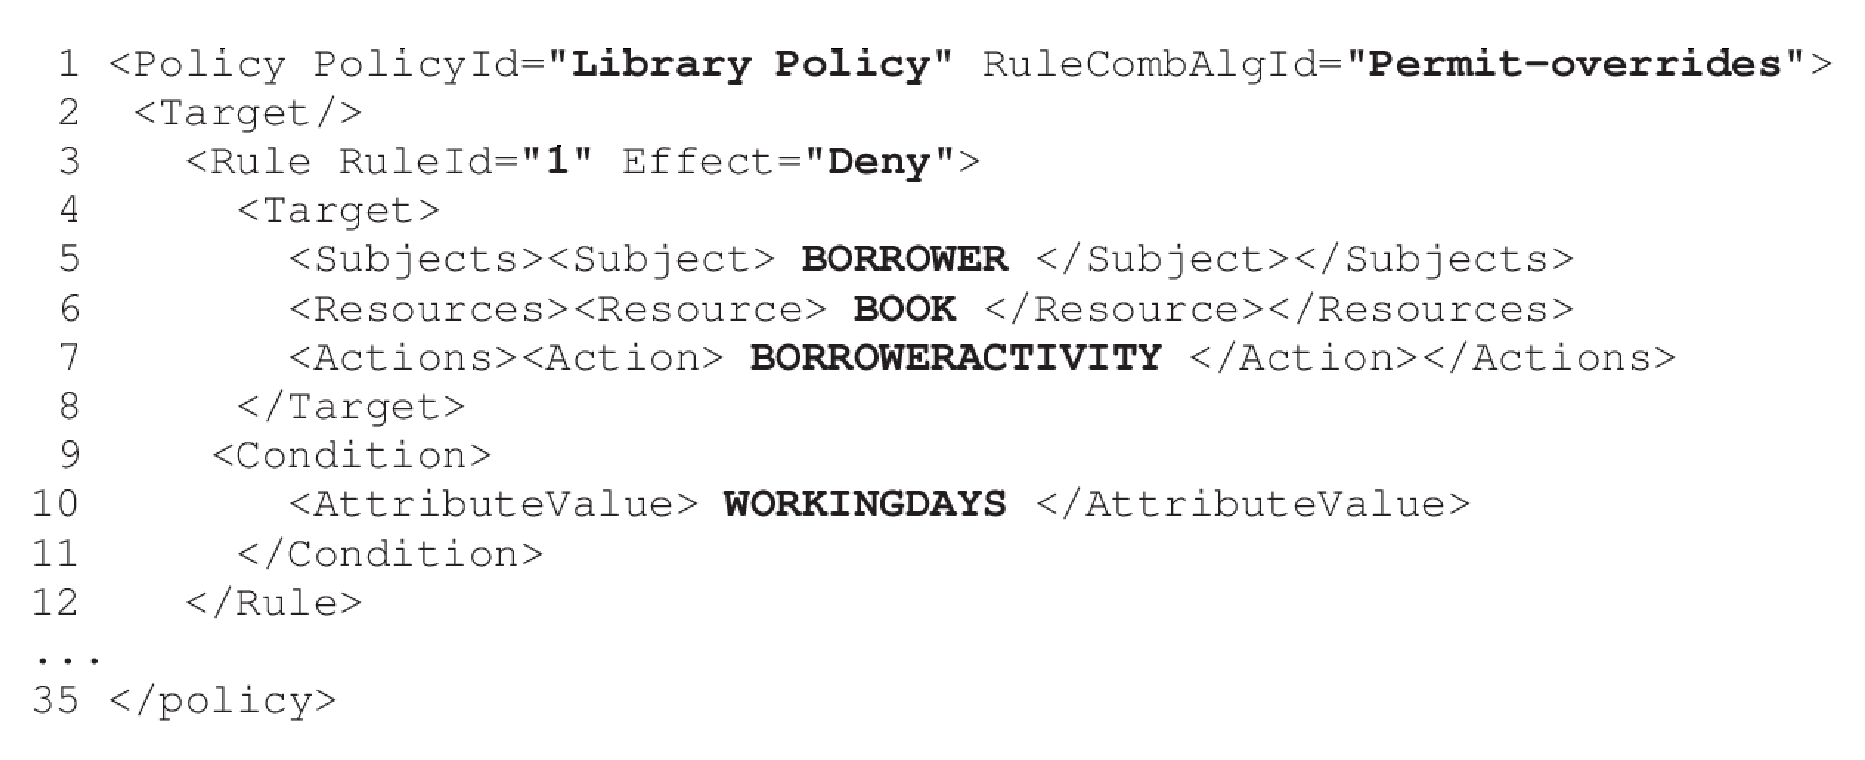
\includegraphics[width=3.5in]{example_mutant.eps}
        \vspace{-5pt}
    \caption{\label{fig:rdcexample}An example mutant policy by changing $R1$'s rule decision (i.e., effect)}
    \vspace{-10pt}
%    \vspace{+3pt}
\end{figure}

%\begin{figure*}[t]%{t}
%\begin{CodeOut}
%\begin{alltt}
% 1 <Policy PolicyId="\textbf{Library Policy}" RuleCombAlgId="\textbf{Permit-overrides}">
% 2  <Target/>
% 3    <Rule RuleId="\textbf{1}" Effect="\textbf{Deny}">
% 4      <Target>
% 5        <Subjects><Subject> \textbf{BORROWER} </Subject></Subjects>
% 6        <Resources><Resource> \textbf{BOOK} </Resource></Resources>
% 7        <Actions><Action> \textbf{BORROWERACTIVITY} </Action></Actions>
% 8      </Target>
% 9	    <Condition>
%10        <AttributeValue> \textbf{WORKINGDAYS} </AttributeValue>
%11      </Condition>
%12    </Rule>
%...
%35 </policy>
%\end{alltt}
%\end{CodeOut}
%\vspace*{-3.0ex} \caption{An example mutant policy by changing $R1$'s rule decision (i.e., effect)}
% \label{fig:rdcexample}
%\end{figure*}


\begin{algorithmic}
\begin{algorithm}[t]
\caption{\label{alg:mutationanalysis}Test Selection based on Mutation Analysis Algorithm}
\STATE{\textit{TestSelection1}($P$, $P_{m}$, $T$): $T'$}
\STATE \textbf{Input:} XACML Policy $P$, modified policy $P_{m}$, Initial Test Cases $T$
\STATE \textbf{Output:} $T' \subseteq T$ where $T'$ is the subset of $T$ selected for use in regression testing $P_{m}$
\STATE {$T'$=\O{}}
\STATE /*Rule-test set-up phase*/
\FOR {each rule $r_{i}$ in Policy $P$}
\STATE {$T_{r_{i}}$=\O{}} where $T_{r_{i}} \subseteq T$ are the tests correlated to $r_{i}$ 
\STATE {/*We mutate the policy $P$ by creating a rule-decision change (RDC) on $r_{i}$ to get $P_{r_{i}}$*/}
\STATE {$P_{r_{i}} \xleftarrow[RDC(r_{i})]{} P$}
\STATE {Execute $T$ with $P_{r_{i}}$}
\FOR {each $t$ in $T$}
\STATE Let $E(t)$ be the test execution result, $E(t)={Success, Failure}$
\IF{$E(t) \leftarrow$ Failure} 
\STATE $T_{r_{i}} \leftarrow T_{r_{i}} \cup t$
\ENDIF
\ENDFOR
\STATE Map($r_{i}$,$T_{r_{i}}$)
\ENDFOR
\STATE /*Test selection phase*/
\STATE $\{r_{m}\}_{i=1..m} \leftarrow diff(P,P_{m})$
\FOR {Each rule $r_{i}$ in $\{r_{m}\}_{i=1..m}$}
\STATE {$T' \leftarrow T' \cup T_{r_{i}}$}
\ENDFOR
\STATE return $T'$
\end{algorithm}
\end{algorithmic}

\subsection{Test Selection based on Mutation Analysis}
Our first proposed test selection technique uses mutation analysis to select test cases as follows. 
The technique needs a preliminary step which is necessary to establish a rule-test correlation.
We next describe rule-test correlation and test selection steps.

\textbf{Rule-Test Correlation Setup.} Given a policy $P$, we create its rule-decision-change (RDC) mutant policy $Pr_i$ by changing decision (e.g., Permit to Deny) of each rule $r_i$ in $P$ in turn.
An example of a mutated policy is shown in Figure~\ref{fig:rdcexample}. In this policy, 
original Rule 1's decision Permit is changed to Deny. The technique finds affected test cases for this rule decision change. 
We execute test cases $T$ on program for $P$ and $Pr_i$. To detect changed policy behaviors, 
the technique monitors responses of evaluated requests formulated from test cases $T$. The test cases, which evaluate different 
policy decisions against $P$ and $P'$, enable to map rule $r_i$ to test cases $t \in T$. The preliminary step ends by establishing 
a correlation between each rule in $P$ and corresponding tests $t \in T$ that trigger this rule.

\textbf{Test Selection.} 
The selection of test cases for regression testing on $P$ and its modified policy $P_m$ starts by conducting change impact analysis 
of $P$ and $P_m$ to find which rules' decision are changed. 
Once these rules are identified, we use the mapping established in the preliminary step to select the subset of 
test cases which are correlated with changed rules.

Algorithm~\ref{alg:mutationanalysis} describes our algorithm used for the technique.
While the technique can quickly select test cases, the technique requires rule-test correlation setup 
(in the preliminary step), which could be costly in terms of execution time. Given n rules in $P$, we execute $T$ for 2$\times$n times. 
As the preliminary step is applied for only existing rules $R$ in $P$, our technique requires addition of rule-test
correlation for newly added rules $R_n$ where $R_n$ $\notin$ $R$ in $P_m$. 
In addition, if a new system test is introduced, we execute this test for 2$\times$n times.
However, an important benefit is that we are enabled to conduct rule-test set-up once before encountering policy 
changes in terms of correlated rules. 


\subsection{Test Selection based on Coverage Analysis}
Our previous technique finds correlation of all of existing rules $N$ in a given policy with the test cases. To reduce
such correlation setup efforts, we develop a technique to correlate only rules, which can be evaluated (i.e., covered)
by test cases. Our intuition is that test cases may interact only with a small number of rules in a policy
instead of all the rules in the policy. We next describe rule-test correlation step.
%We do not describe test selection step, which is identical to the preceding technique.


\begin{algorithmic}
\begin{algorithm}[t]
\caption{\label{alg:coverageanalysis}Test Selection based on Coverage Analysis Algorithm}
\STATE{\textit{TestSelection2}($P$, $P_{m}$, $T$): $T'$}
\STATE \textbf{Input:} XACML Policy $P$, modified policy $P_{m}$, Initial Test Cases $T$
\STATE \textbf{Output:} $T' \subseteq T$ where $T'$ is the subset of $T$ selected for use in regression testing $P_{m}$
\STATE {$T'$=\O{}}
\STATE /*Rule-test set-up phase*/
\FOR {Each test case $t$ in $T$}
\STATE {Execute $t$ with $P$}
\STATE $MAP$=Map($t$,$\{r_{p}\}_{i=1..p}$) where $\{r_{p}\}_{i=1..p}$ are the rules in $P$ that are evaluated (i.e., covered) by $t$
\ENDFOR
%\STATE Generate a mapping rule/test from $MAP_{1}$
%\STATE $MAP_{2}$=Map($r_{i}$,$T_{r_{i}}) \leftarrow MAP_{1}$
\STATE /*Test selection phase*/
\STATE $\{r_{m}\}_{i=1..m} \leftarrow diff(P,P_{m})$
\FOR {Each rule $r_{i}$ in $\{r_{m}\}_{i=1..m}$}
\STATE {$T' \leftarrow T' \cup T_{r_{i}}$}
\ENDFOR
\STATE return $T'$
\end{algorithm}
\end{algorithmic}

\textbf{Rule-Test Correlation Setup.} Given a policy $P$,
Thus we execute test cases $T$ on program that interacts with $P$. Our technique monitors which rules in a policy are evaluated with
requests formulated from test cases $T$. Then, we establish correlation between test cases and evaluated (i.e., covered) rules in $P$. 

%\textbf{Test Selection.} 
%The selection of test cases for regression on $P$ and its modified policy $P_m$ starts by conducting change impact analysis 
%of $P$ and $P_m$ to find which rules' decision are changed. 
%Once these rules are identified, we use the mapping established in the preliminary step to select the subset of 
%test cases which are correlated with changed rules.
\textbf{Test Selection.}
Once the mapping test-rule is established, we proceed test selection step described in the first approach with
the results of change impact analysis of $P$ and $P_m$. The results include information to show which rules' decision have changed.
This test selection maps test cases with those rules to constitute the subset of existing test cases.

Algorithm~\ref{alg:coverageanalysis} describes our algorithm used for the technique.
An important benefit of this technique is to reduce cost in terms of mutation analysis and execution time. This technique does not 
require generating mutants by changing rule's decision in turn. Moreover, the technique can significantly reduce execution time.
While the technique can quickly select system tests in the second step, the technique requires rule-test correlation setup (in the preliminary step), 
which could be costly in terms of execution time. Consider that requests $Rs$ are formulated from test cases interact 
only n$_1$ rules (n$_1$ $\leq$ n) in a policy.
We execute $T$ only once. Our technique requires addition of rule-test
correlation for newly added rules $R_n$ where $R_n$ $\notin$ $R$ in $P_m$ as the same with the previous technique.


\begin{algorithmic}
\begin{algorithm}[t]
\caption{\label{alg:reqevaluation}Test Selection based on Recorded Request Evaluation}
\STATE{\textit{TestSelection3}($P$, $P_{m}$, $T$): $T'$}
\STATE \textbf{Input:} XACML Policy $P$, modified policy $P_{m}$, Initial Test Cases $T$
\STATE \textbf{Output:} $T' \subseteq T$ where $T'$ is the subset of $T$ selected for use in regression testing $P_{m}$
\STATE {$T'$=\O{}}
\STATE {$R_{T'}$=\O{}} where $R_{T'}$ are the requests corresponding to $T'$ 
\STATE {Execute system requests $R$}
\FOR {each request $Re$ in $R$}
\IF {$decision(Re/_{P}) \neq decision(Re/_{P_{m})}$}
\STATE {$R_{T'} \leftarrow R_{T'} \cup Re$}
\ENDIF
\ENDFOR
\STATE {$T' \leftarrow R_{T'}$}
\STATE return $T'$
\end{algorithm}
\end{algorithmic}

\subsection{Test Selection based on Recorded Request Evaluation}
To reduce such correlation setup efforts in the previous techniques, we develop
a technique, which does not require rule-test correlation setup.
Instead of correlation, our technique records test cases and their issued requests as a preliminary step.
More specifically, our technique executes test cases $T$ on a program for $P$ and records all requests issued to policy decision point (PDP) for each test case. For test selection, our technique evaluates all issued requests against $P$ and $P_m$ and selects the test subset of
requests (with corresponding system test cases) that engender different decisions for two different policy versions.

%While our previous two techniques require correlation rule-test setup. 
%The techniques analyze two versions of policies statically 
%or dynamically under test to find which rules' are changed. However, these technique require correlation setup.
Algorithm~\ref{alg:reqevaluation} describes our algorithm used for the technique.
The current approach requires the execution of system test cases $T$ only once.
% For additional test cases, we execute the tests only once. 
Moreover, while the two previous techniques are white-box testing since access control policies are available, the present technique 
does not require the availability of access control policies. This can present a considerable advantage when developers don't want 
to reveal their access control policies.



\subsection{Test Augmentation}
\label{subsec:testaugmentation}
While test-selection techniques are useful for selecting test cases for a program impacted by policy changes, these test cases may not sufficiently cover all the rules in the policy impacted by the changes.
We develop a test augmentation technique, which complements our test-selection techniques by generating additional test cases to 
cover not-covered-impacted-rules $N_r$ by existing test cases.

Our augmentation technique first analyzes change impact analysis between $P$ and $P'$ to find rules impacted by policy changes.
The technique finds $N_r$ by evaluating selected test cases and monitoring which 
rules are evaluated during test case execution.
%our selected test cases and $P$ and $P'$. 
For $N_r$, we next generate requests, which can cover $N_r$.
We then analyze existing test cases to create test cases, which issue the requests
to cover $N_r$ with minimal changes in test cases.
For example, attribute change (e.g., subject element change from $Student$ to $Professor$) may cover $N_r$. We then verify that augmented test cases increase coverage of $N_r$.
%[TBD]

%\textbf{Distance-based complexity: Besides the simple graph 
%complexity, we extract distance-based complexity measures 
%based on the shortest distance between all pairs of crash 
%graph nodes using the Floyd-Warshalls algorithm  [7]. The 
%initial distance between two connected nodes is set to 1. 
%Then, we compute distance-based complexities such as 
%eccentricity, density and radius. For example, the eccentricity 
%of a node v is the greatest distance between v and any other 
%node. We aggregate all eccentricities with minimum 
%(=radius), maximum (=diameter) and average. Table III 
%describes selected features, while detailed measures are 
%described in [21].}








